\documentclass{article}

\usepackage{geometry}
\geometry{a4paper, portrait, margin=1.5in}

\usepackage{hyperref}
\hypersetup{
    colorlinks=true,
    linkcolor=black,
    filecolor=magenta,
    urlcolor=blue,
}

\usepackage{graphicx}
\graphicspath{ {images/} }

\usepackage{tcolorbox}
\usepackage{textcomp}
\usepackage{gensymb}
\usepackage{indentfirst}

\title{Autodesk Eagle CAD Guide}
\author{Evan Peterson}
\begin{document}
\maketitle{}
\setcounter{tocdepth}{2}
\tableofcontents
\pagebreak

\section{Introduction}

\subsection{What is a PCB}
A printed circuit board (PCB) is used to mechanically support and electrically connect various electrical components. A PCB is designed and manufactured based on how you want to connect the components then the components are soldered to the PCB. \par
In its most basic form a PCB consists of a center substrate (typically fr4) with a layer of copper traces on the bottom and top. Pads are portions of the copper layer that are in specific shapes so a component can be soldered to it.

\subsection{Eagle Intro}
Eagle is a CAD tool used to design printed circuit boards (PCBs). The program is split up into three sections which build upon one another to result in files that are sent to a PCB manufacturer.\par
First all parts to go on the board are created in libraries which describe the pins on the part and the footprint of the part for when it is soldered to the board. Then these parts are used in the Schematic design which describes the electrical connections on the board. Then the board is laid out by following the parts and connections made in the schematic to place parts on the physical board then route where the physical connections will go between parts.
\begin{tcolorbox} [title=Tips \& Tricks]
    \begin{itemize}
        \item Everything in Eagle can be done through clicking buttons or by using its command line. Design can be done much quicker by learning to use the command line.
        \item In order to use some Eagle functions such as creating new files or adjusting certain settings you must switch back to Eagle's Control Panel window
    \end{itemize}
\end{tcolorbox}

\subsection{Eagle Installation}
\begin{enumerate}
    \item Download at \url{www.autodesk.com/products/eagle}
    \item Install Eagle using free or educational version
    \begin{itemize}
        \item Free version: 2 Board Layers, 80cm\textsuperscript{2} Board Area
        \item Educational version: 16 Board Layers, Unlimited Board Area
        \begin{itemize}
            \item \url{www.autodesk.com/education/free-software/eagle}
        \end{itemize}
    \end{itemize}
\end{enumerate}

\section{Libraries}
Libraries are used to store information about a part which are used in the schematic and the board layout. Eagle has built in libraries for many common parts but very often you have to make your own. \par
Libraries are split into three parts. The Symbol is what is seen in the schematic and is how you describe the pins on your part which electrical connections go to. The Package is the footprint used for board layout which you will solder the component to on the physical board. The Device brings the Symbol and Package together so what is created in the schematic can be translated into the board layout.

\subsection{Create Library} \label{create library}
\begin{enumerate}
    \item (At Control Panel) \textit{\textbf{File\textrightarrow
    New\textrightarrow Library}}
    \item Save to a directory where you will keep all Eagle libraries
\end{enumerate}
\begin{tcolorbox} [title=Tips \& Tricks]
    \begin{itemize}
        \item Libraries are commonly split up into components types such as resistors or connectors
        \item Eagle has a default folder it searches for its libraries, but you can have it search additional folders for your libraries by (At Control Panel) \textit{\textbf{File\textrightarrow Options\textrightarrow Directories}} then appending to the Libraries path a colon then the path to your directory
    \end{itemize}
\end{tcolorbox}

\subsection{Library Part: Symbol}
\begin{enumerate}
    \item Create new symbol: \textit{\textbf{Library\textrightarrow Symbol}}
    \item Name symbol with part number
    \item Draw box using \textit{\textbf{wire}}
    \begin{itemize}
        \item This aspect is purely visual so any size/shape is okay, but use standard symbols which are commonly represented in schematics
    \end{itemize}
    \item Add necessary amount of pins using \textit{\textbf{pin}}
    \begin{itemize}
        \item These pins are what wires are connected to in the schematic
    \end{itemize}
    \item Name pins corresponding to datasheet using \textit{\textbf{name}} then click on pin
    \item Clean up Symbol: Adjust part outline so all pins fit and pin names can be seen
    \item Add Name and Value using \textit{\textbf{text}}
    \begin{itemize}
        \item \textgreater NAME and  \textgreater VALUE are keywords for text that are automatically filled out with the name and value when inserted into a schematic.
    \end{itemize}
    \item Change Layer of Name and Value using \textit{\textbf{info}} then clicking on the part and changing Layer to Name and Value respectivly
    \item Return to Library: \textit{\textbf{Library\textrightarrow Table of Contents}}
\end{enumerate}

\begin{figure}[!h]
    \center
    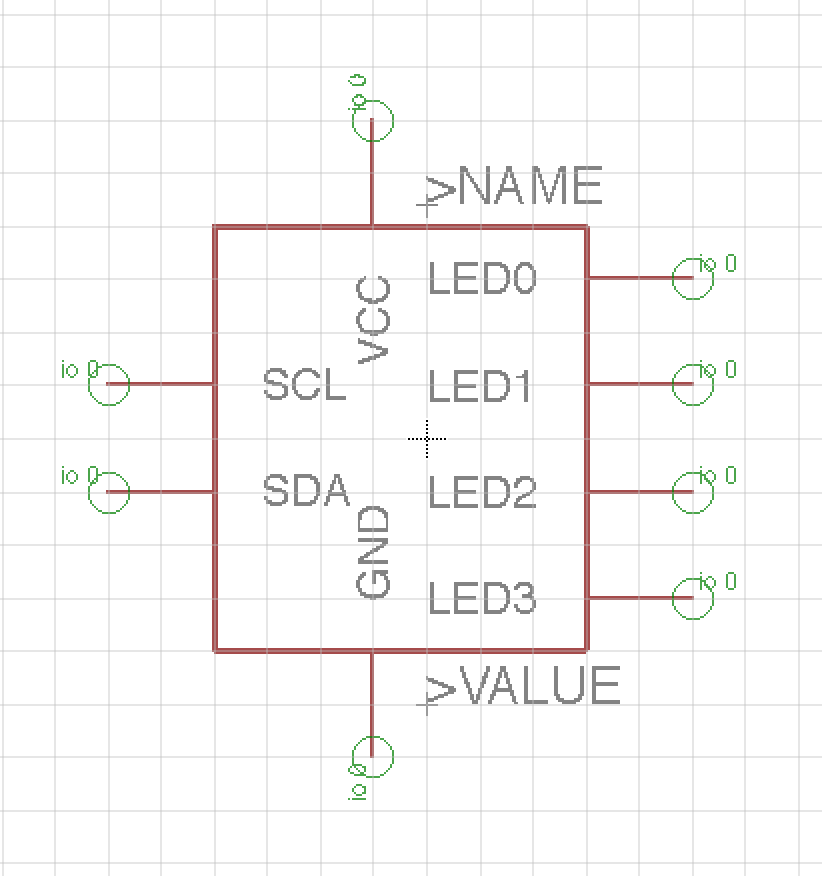
\includegraphics[width=0.4\textwidth,height=0.4\textheight,keepaspectratio]{symbol}
    \caption {Example of completed symbol}
    \label{img:symbol}
\end{figure}

\begin{tcolorbox} [title=Tips \& Tricks]
    \begin{itemize}
        \item Always keep pins snapped to the 0.1 in grid
        \item Right click while placing or moving to rotate
        \item To move a group use \textit{\textbf{group}}, select what you want to move then \textit{\textbf{Right Click\textrightarrow Move:Group}}
        \item Objects are clickable and selectable from the grey +
    \end{itemize}
\end{tcolorbox}

\subsection{Library Part: Package}
This is typically the footprint for the package which is found in the datasheet for the part. In the datasheet you will find all measurements needed to create the package. This package will go on the PCB and is what the component will be soldered to.
\begin{enumerate}
    \item Create new package: \textit{\textbf{Library\textrightarrow Package}}
    \item Name package with package name
    \begin{itemize}
        \item Common for multiple parts to have the same package
    \end{itemize}
    \item Place first pad
    \begin{itemize}
        \item Place surface mount using \textit{\textbf{SMD}}
        \item Place through hole pad using \textit{\textbf{pad}}
    \end{itemize}
    \item Resize pad using \textit{\textbf{info}} clicking on pad then changing SMD size to size given in datasheet
    \item Use \textit{\textbf{copy}} to copy correct amount of pads and place them in approximate positions
    \item Use values given in datasheet to calculate position (to pad center) for each pad then move pads using \textit{\textbf{info}} and change position values
    \item Rename pads using \textit{\textbf{rename}}. Pad numbers given by datasheet
    \item Add part outline using \textit{\textbf{line}} then changing Layer dropdown to \textit{\textbf{51 tDocu}} then draw basic part outline
    \begin{itemize}
        \item The tDocu is just for reference to ensure no overlapping parts so it will not appear on the board.
    \end{itemize}
    \item Adjust part outline to the dimmensions given on the datasheet. Adjust to exact values using \textit{\textbf{info}}
    \item Add silkscreen
    \begin{itemize}
        \item Silkscreen gets printed on the board and is used to help place components
        \item Draw lines on the \textit{\textbf{21 tPlace}} layer as an outline that does not intersect with pads
        \item Add a dot to indicate where Pin 1 is on component to help when soldering component
    \end{itemize}
    \item Add Name and Value using \textit{\textbf{text}}
    \begin{itemize}
        \item Use \textgreater NAME and  \textgreater VALUE similar to in symbol
        \item Adjust Layer to Name and Value respectivly
    \end{itemize}
    \item Return to Library: \textit{\textbf{Library\textrightarrow Table
    of Contents}}
\end{enumerate}
\begin{tcolorbox} [title=Tips \& Tricks]
    \begin{itemize}
        \item Change grid size using \textit{\textbf{grid}}
        \begin{itemize}
            \item Change grid size to whatever is helpful to you
            \item Use same units as given in datasheet. Values for position and size are in these units
            \item Recommended: Size = 0.5mm, Alt = 0.25mm
        \end{itemize}
        \item Use positions such that (0,0) is at the center of the component
    \end{itemize}
\end{tcolorbox}

\begin{figure}[!h]
    \center
    \includegraphics[width=0.4\textwidth,height=0.4\textheight,keepaspectratio]{package}
    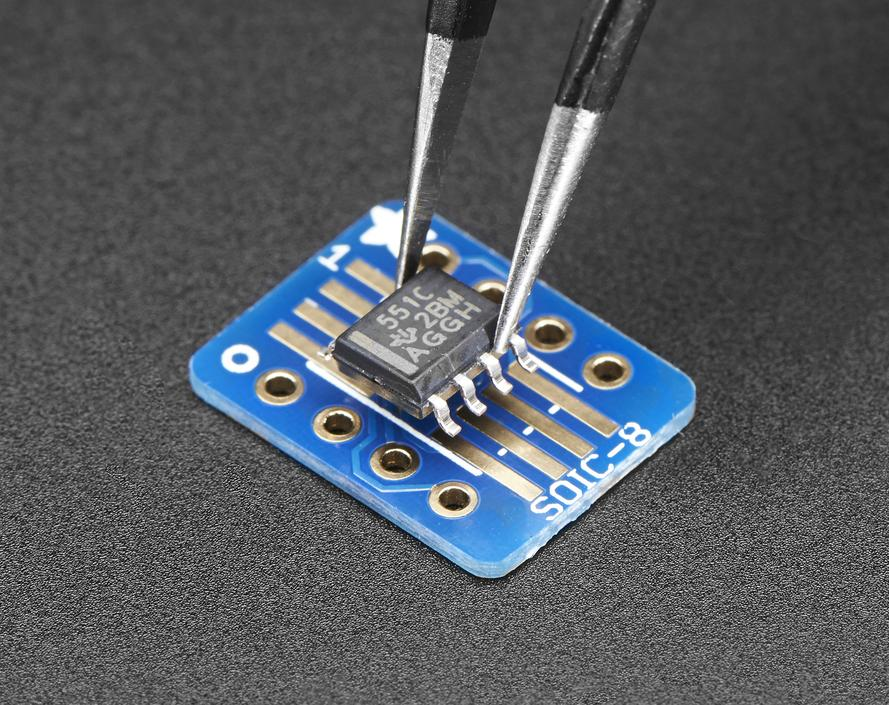
\includegraphics[width=0.5\textwidth,height=0.5\textheight,keepaspectratio]{package2}
    \caption {Example of completed package and how the physical component goes on a package that was created}
    \label{img:package1}
\end{figure}

\subsection{Library Part: Device}
This is where the Symbol and Package come together to create what will be added to the schematic.
\begin{enumerate}
    \item Create new device: \textit{\textbf{Library\textrightarrow Device}}
    \item Name with general part number
    \begin{itemize}
        \item Not package specific because a single device can have multiple packages
    \end{itemize}
    \item Add symbol using \textit{\textbf{add}} then select previously created symbol
    \item Place symbol so grey + is in center of component
    \item Click new button in package window and select previously created package
    \item Connect pins by clicking connect button in package area
    \item Use datasheet to see what pin names correspond to what pad numbers then connect by selecting pin and pad then click connect. Repeat for each one
    \item Click prefix button to add current prefix to match component type
\end{enumerate}
\begin{tcolorbox} [title=Tips \& Tricks]
    \begin{itemize}
        \item A wildcard character \textit{\textbf{*}} can be used in Device name to allow you have names for different versions of the part without creating a new device. Example: You have parts A45C and A46C that have the same pins and package, but have some minor internal difference. You can name device A4*C then specify two technologies: 5 and 6.
        \item You can add multiple packages and set the variant name to specify the package. This variant name is appended to the end of the Device name
    \end{itemize}
\end{tcolorbox}

\begin{itemize}
    \item Done with library part and ready to be added to schematic
    \item Many more parts can be added to this library. Parts that share packages only need package to be created once so check if that package exists first so you don't have to remake it.
\end{itemize}

\section{Schematic}
Schematics are used to set up how the board is organized by adding all the parts used on the board and making the electrical connections between these parts.
\begin{enumerate}
    \item (At Control Panel) \textit{\textbf{File\textrightarrow New\textrightarrow Schematic}}
    \item Save to a directory where you are storing this project
\end{enumerate}
\begin{tcolorbox} [title=Tips \& Tricks]
    \begin{itemize}
        \item Always keep parts and wires snapped to 0.1 in grid
    \end{itemize}
\end{tcolorbox}

\subsection{Schematic: Adding Parts}
\begin{enumerate}
    \item Prepare Eagle with necessary libraries
    \begin{itemize}
        \item Libraries can be added by automatically searching a folder as shown in section \ref{create library}
        \item Libraries can also be temporarily added by \textit{\textbf{Library\textrightarrow Use}} then select library you created
    \end{itemize}
    \item Add components using \textit{\textbf{add}} then select the library containing the component then select the component
    \begin{itemize}
        \item Add a frame to keep schematic organized
        \item Add all components needed for schematic
        \item Resistors and Capacitors are found in rcl library. R-US and C-US are the parts commonly used and the SMD package 0603 is commonly used (parts named R-US\_R0603 and C-USC0603 respectively)
    \end{itemize}
    \item Change value of parts using \textit{\textbf{value}}
    \begin{itemize}
        \item This value has no effect on the board, only used as reference
    \end{itemize}
\end{enumerate}
\begin{tcolorbox} [title=Tips \& Tricks]
    \begin{itemize}
        \item When adding components you can search for components but Eagle uses exact matching so you must add wild cards. Example: you want to search for part number containing 0603, search using *0603*
    \end{itemize}
\end{tcolorbox}

\subsection{Schematic: Wiring}
\begin{enumerate}
    \item Organize components
    \begin{itemize}
        \item Components need to be placed in a way so it is easy to read
    \end{itemize}
    \item Use the net tool draw connections between components
    \begin{itemize}
        \item NOT the wire tool. The wire tool is only used for visuals, does not make any actual connections
    \end{itemize}
    \item Connect power and ground using parts from the supply library. All supply parts that are the same on a schematic are connected together
    \begin{itemize}
        \item Good practice to have ground supply parts pointing down and power supply parts pointing up
    \end{itemize}
\end{enumerate}
\begin{tcolorbox} [title=Tips \& Tricks]
    \begin{itemize}
        \item Connections can be made without running nets between components. This is done by using \textit{\textbf{name}} on a multiple nets and naming them the same thing. All nets with the same name are treated as being connected.
        \begin{itemize}
            \item Pins cannot be named, add a short net connecting to the pin then name that net
            \item Name these nets something useful so it is easier to follow
            \item To see that nets are named the same and connected, you can use \textit{\textbf{label}} on a net and place the label at the end of the net
        \end{itemize}
        \item Connections can be checked with \textit{\textbf{show}}
    \end{itemize}
\end{tcolorbox}

\subsection{Schematic: Error Checking}
\begin{itemize}
    \item Use the Electrical Rule Check (ERC) to check for electrical errors
    and warnings
    \item The ERC is often useful to show connections you missed
    \item Many warnings can be ignored from the ERC because they often have to do with net names, etc.
\end{itemize}

\section{Board Layout}
The board file is how you layout the final physical board. All steps up to this point have been to assist you in the creation of this.
\begin{enumerate}
    \item When done with schematic switch to board by
    \textit{\textbf{File\textrightarrow Use}}
    \begin{itemize}
        \item If no board file is found one will be generated
        \item It is generated with parts from the schematic randomly placed and lines showing the connections to be made between parts called airwires
    \end{itemize}
\end{enumerate}

\subsection{Board Layout: Layers}
\begin{itemize}
    \item What is actually printed:
    \begin{itemize}
        \item Top Silkscreen (printed on top of board for reference, typically white)
        \item Top Soldermask (applied over copper to protect from solder, typically green)
        \item Top Copper (makes electrical connections and components are soldered to)
        \item Substrate (FR4: used to support and separate copper layers)
        \item Bottom Copper
        \item Bottom Soldermask
        \item Bottom Soldermask
    \end{itemize}
    \item Use \textit{\textbf{layer}} to adjust what layers are currently viewed
\end{itemize}
\begin{tcolorbox} [title=Tips \& Tricks]
    \begin{itemize}
        \item Right click on Layer settings to create a group of currently viewable layers or quickly switch between created groups
    \end{itemize}
\end{tcolorbox}

\begin{figure}[!h]
    \center
    \includegraphics[width=0.4\textwidth,height=0.4\textheight,keepaspectratio]{layers}
    \caption {Sideview of layers that are created when PCB is manufactured}
    \label{img:layers}
\end{figure}

\subsection{Board Layout: Arranging}
\begin{itemize}
    \item Use \textit{\textbf{move}} and right click to rotate
    \item How you arrange your parts has a large impact on the routing difficulty in the next step
    \item First consider the requirements of your board
    \begin{itemize}
        \item Consider the maximize size you want your board to be
        \item Consider Location of specific parts
        \begin{itemize}
            \item Specific locations of connectors and other components that need to be accessible
            \item Decoupling capacitors very close to its IC
            \item Maximum distances parts can be that must communicate
        \end{itemize}
        \item Consider mounting holes
        \item Consider clearance with other boards or objects around it
    \end{itemize}
    \item Then consider what is easiest placement for when you route the board
    \begin{itemize}
        \item Leave space between parts so no parts collide and so you have enough space for routing
        \item Group parts together based on function, referring back to schematic. Reduces required routing distances
        \item Minimize intersecting airwires. It is much more difficult to route when airwires cross
        \item Recommended keeping as many components as you can on the top layer so you can use the bottom layer for routing or ground plane
    \end{itemize}
    \item Use \textit{\textbf{delete}} to erase existing dimension then use
    \textit{\textbf{wire}} with the layer set to \textit{\textbf{20 Dimmension}} then draw a new dimension which all your parts are within
\end{itemize}

\subsection{Board Layout: Routing}
\begin{itemize}
    \item Routing is making all the connections shown by the airwires without overlapping anything
    \item Two layer board so you can place components and route on the top or the bottom
    \begin{itemize}
        \item Vias are used to connect between the top and bottom layers
    \end{itemize}
    \item Don't worry about ground connections yet, a ground plane will be added later
    \item Use \textit{\textbf{route}} (not \textit{\textbf{wire}})
    \begin{itemize}
        \item Use layer dropdown to select signal layer you are routing on
        \item Optional selection for walkaround obstacles to assist you with routing to avoid overlapping based on DRC rules
        \item Bend style is the angle of wires when routing (good practice to use 45\degree\ angles)
        \item Width is how wide the copper trace is (recommended 0.3mm)
        \begin{itemize}
            \item Trace width must be considered for some applications such as power lines
        \end{itemize}
        \item Via settings are for size and shape of via (recommended circle with drill of 0.35mm)
    \end{itemize}
    \item Start from end of an air wire and route to the other end of that airwire
    \item Left click when routing to place segment and continue routing
    \item Ensure no overlap when routing
    \begin{itemize}
        \item For pads and traces on the same layer there must be zero overlap
        \item Traces on separate layers can overlap
        \item Vias and through hole components (colored in green) are on both layers so traces cannot overlap with these on either layer
    \end{itemize}
    \item Vias can be added by changing layers while routing (using middle click) or by adding manually with the via tool
    \begin{itemize}
        \item Vias added manually do not have the net automatically set so must use \textit{\textbf{name}} to change name of via to same as net you want to connect it to
    \end{itemize}
    \item Different PCB manufacturers have specifications for the minimum distance they can produce between traces
    \begin{itemize}
        \item You must ensure your traces are at least that far apart
    \end{itemize}
    \item Traces and vias cannot be removed with \textit{\textbf{delete}}, you must use \textit{\textbf{ripup}}
    % add about bus routing
\end{itemize}
\begin{tcolorbox} [title=Tips \& Tricks]
    \begin{itemize}
        \item Right click while routing to switch bend styles
        \item Use \textit{\textbf{ratsnest}} to recalculate airwires to shortest
        length
    \end{itemize}
\end{tcolorbox}

\begin{figure}[!h]
    \center
    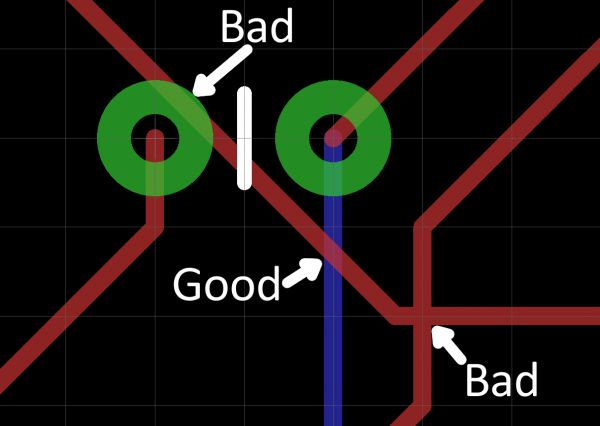
\includegraphics[width=0.4\textwidth,height=0.4\textheight,keepaspectratio]{routing}
    \caption {Example of allowable routing connections}
    \label{img:routing}
\end{figure}

\subsection{Board Layout: Polygons}
Polygons are how large sections of copper (like ground planes) are done. Using a ground plane allows you to connect many ground pins without routing as well as other benefits.
\begin{enumerate}
    \item Use \textit{\textbf{polygon}} to draw the shape around you want to
    fill
    \begin{itemize}
        \item For ground plane you typically want to fill the whole board so draw the polygon along the dimension lines
    \end{itemize}
    \item Use \textit{\textbf{name}} to connect this polygon to the net with the same name
    \item Use \textit{\textbf{ratsnest}} to fill in the polygons
\end{enumerate}
\begin{tcolorbox} [title=Tips \& Tricks]
    \begin{itemize}
        \item Change the polygon's rank when you have intersecting polygons to give one higher priority
        \item Add polygon inside of another and change Polygon pour to cutout if there is a section of the board you don't want a polygon
        \item Check or uncheck thermals based on application (typically good idea to use when polygon overlaps pads so the component is easier to solder on)
    \end{itemize}
\end{tcolorbox}

\begin{figure}[!h]
    \center
    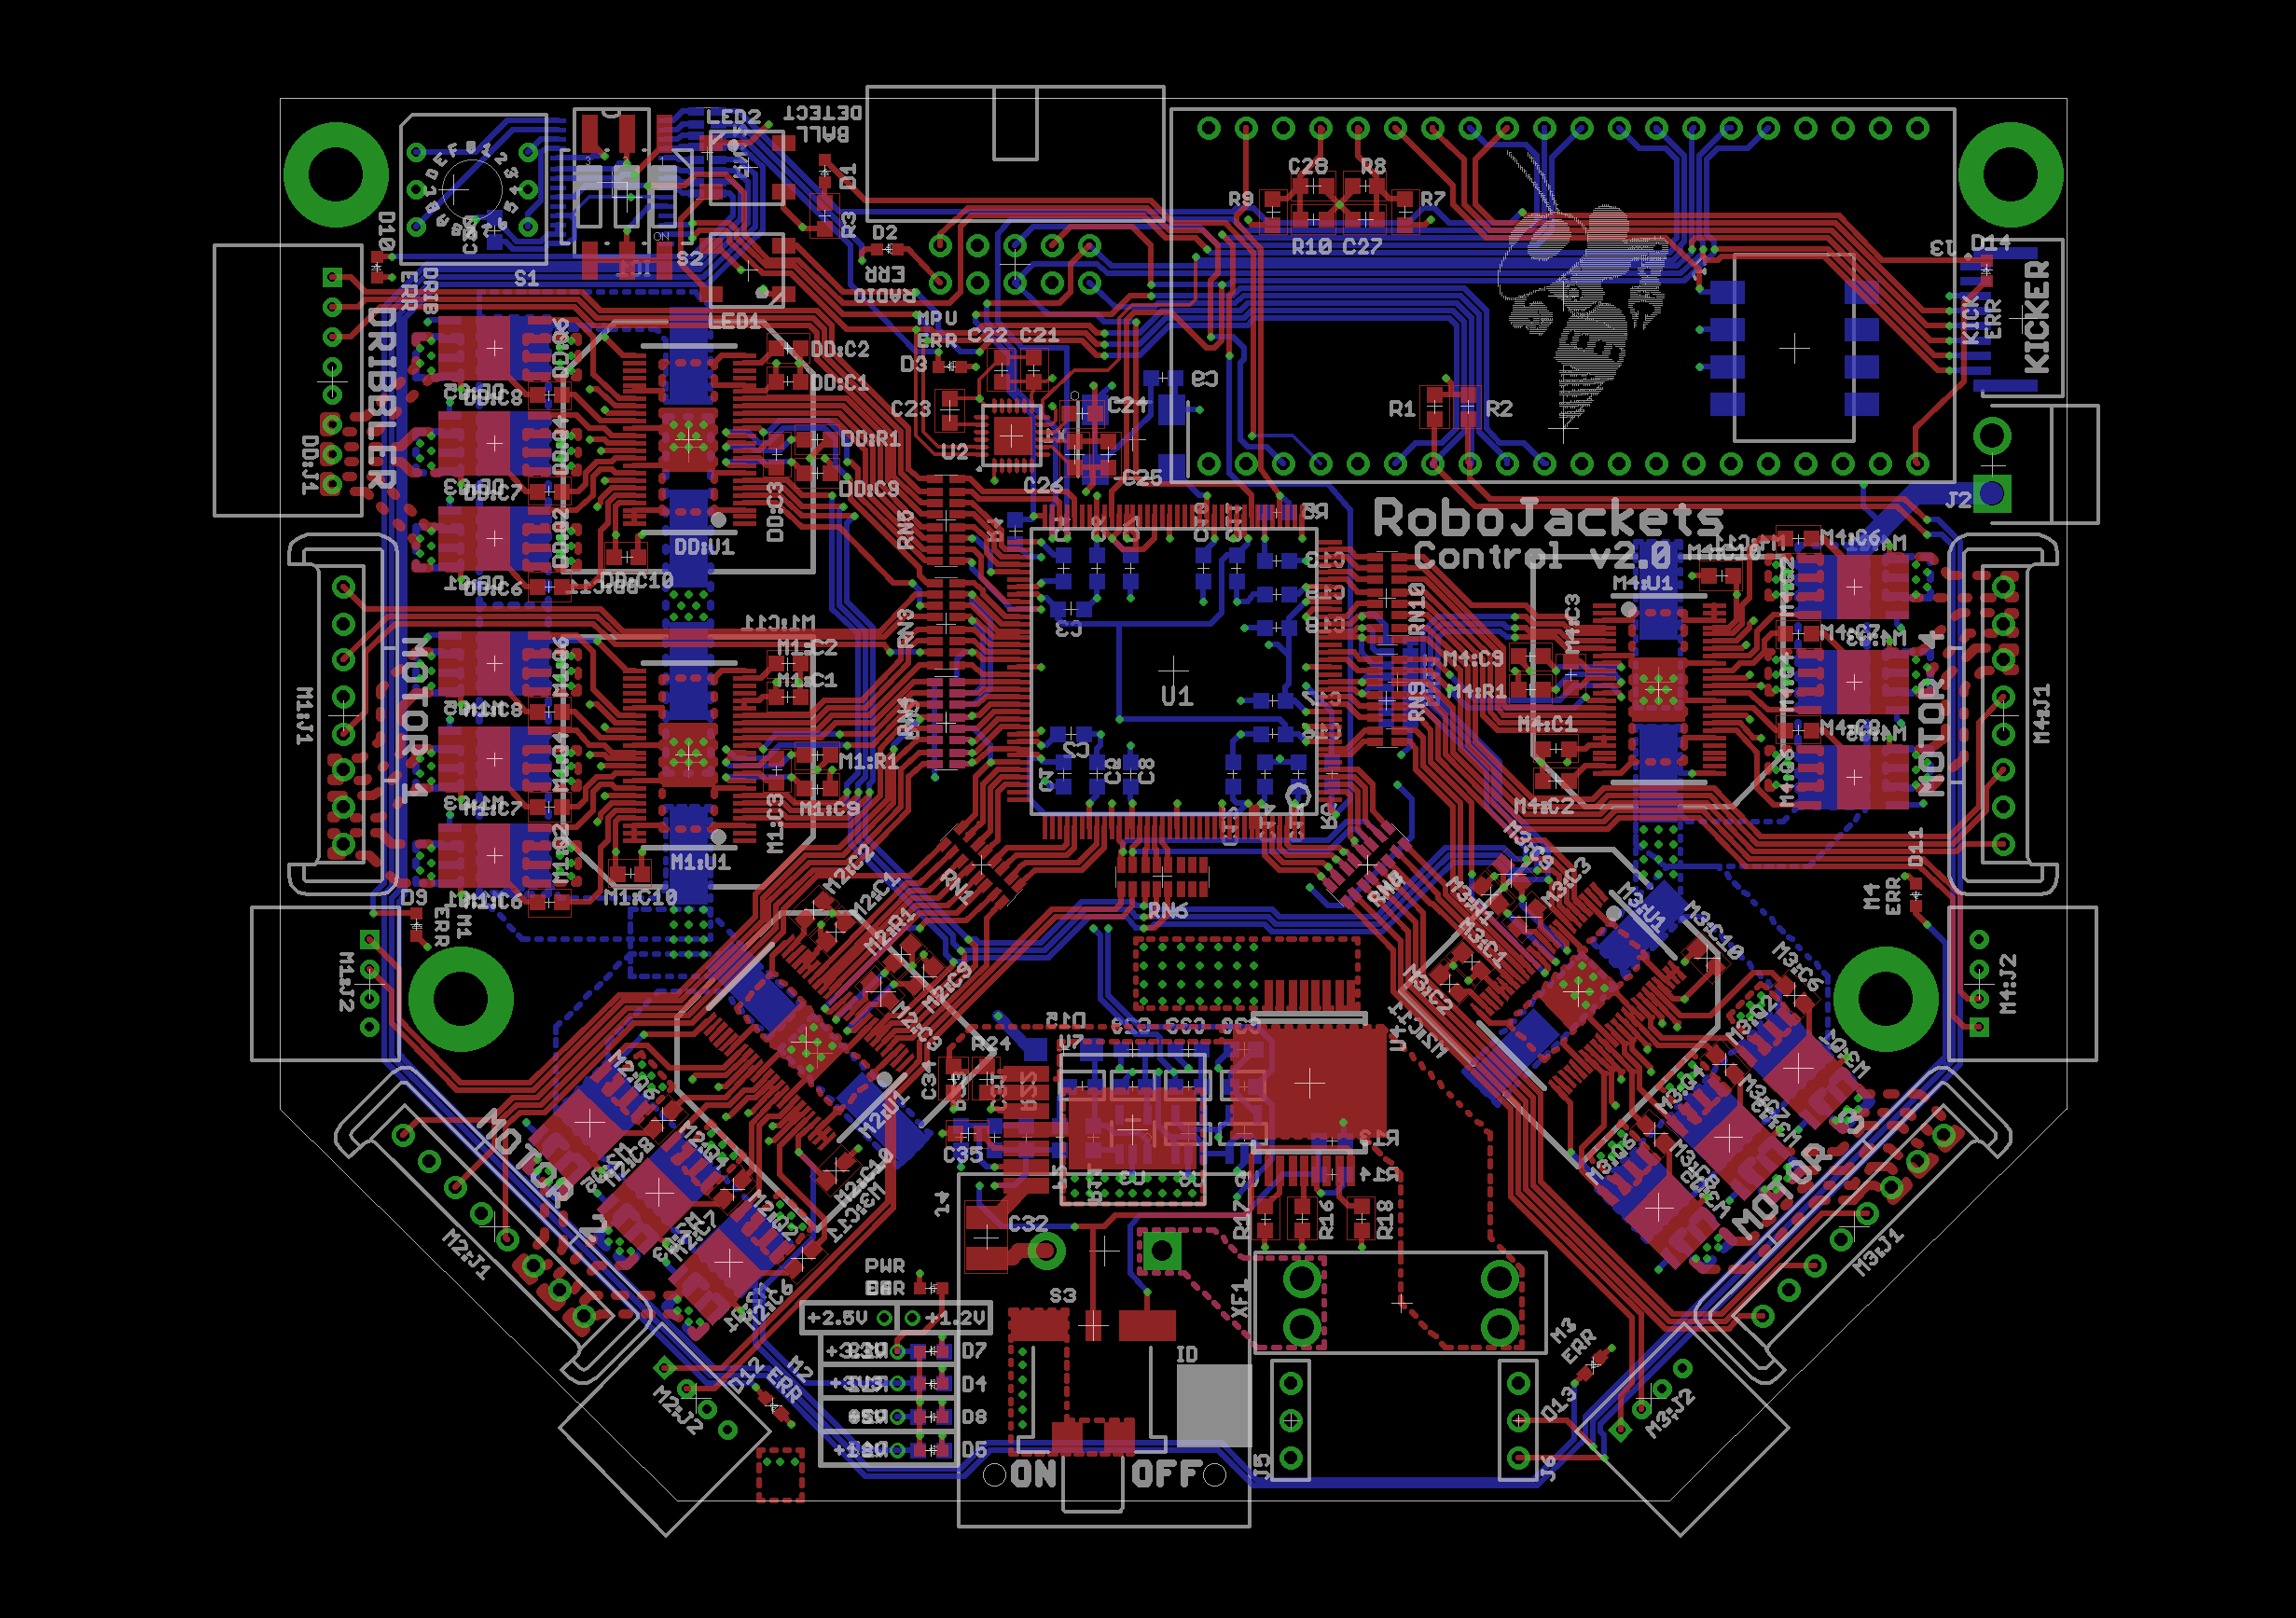
\includegraphics[width=0.8\textwidth,height=0.6\textheight,keepaspectratio]{control}
    \caption {Example of fully completed board}
    \label{img:control}
\end{figure}

\subsection{Board Layout: Silkscreen}
\begin{itemize}
    \item Silkscreen is printed on the top and bottom of the board and has no effect on the function of the board. Rather it is used to identify parts on the board and to help with component soldering.
    \item Most of the silkscreen comes from individual parts on Names layer identifying part names
    \item Often these names for parts are misaligned. Use
    \textit{\textbf{smash}} on the component to allow you to move these labels
    \item Add other markings to silkscreen on layers tPlace or bPlace for the top and bottom silkscreen respectively
\end{itemize}

\subsection{Board Layout: Error Checking}
\begin{itemize}
    \item Use \textit{\textbf{ratsnest}} then check the notification at the bottom left for how many airwires are left to see if there is stuff left to route. Everything is routed if "Nothing to do"
    \item Use the Design Rule Check (DRC) to check for clearance, overlap, etc
    \item Settings of DRC can be changed to fit the requirements of where your board is being printed
    \item When "Ratsnest: Nothing to do" and "DRC: No errors" you are done
\end{itemize}

\subsection{Board Layout: Exporting}
You must export the board into Gerber files which are sent to the manufacturer to print. This is a set up multiple files, one for each layer
\begin{enumerate}
    \item Use \textit{\textbf{File\textrightarrow CAM Processor}} then \textit{\textbf{File\textrightarrow Open\textrightarrow Job}} and select gerb274.cam
    \begin{itemize}
        \item There is also a 4 layer version of this CAM
    \end{itemize}
    \item This exports a file for each layer with the exception of of bottom silkscreen. This can be added if desired by clicking add and selecting Dimension, bPlace, and bNames
    \item Repeat CAM Processor with excellon.cam job to generate drill file
\end{enumerate}
% \subsection{Layers}
% reference Prefixes
% reference Layers
% reference Commands

% \section{Ordering}
% \section{Soldering}
\end{document}